\section{Half-wave Rectifier}

Trong bài tập này, một nguồn xoay chiều được sử dụng để tạo ra đầu ra chỉnh lưu nửa sóng bằng cách sử dụng một diode. Sơ đồ mô phỏng được đưa ra dưới đây:

\begin{figure}[h]
    \centering
    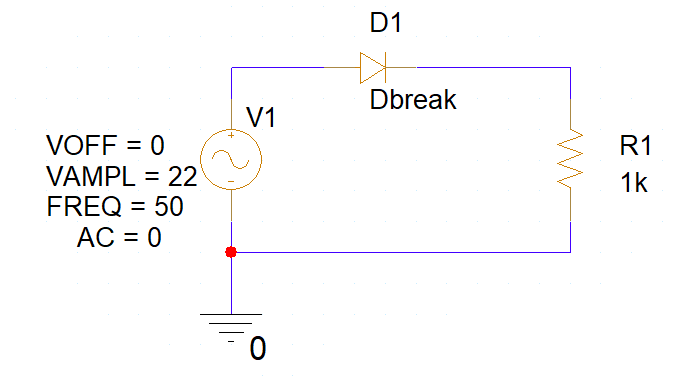
\includegraphics[width=0.7\textwidth]{graphics/ex6/f1.PNG}
    \caption{Half-wave Rectifier with Voltage Sin Source}
\end{figure}

\subsection{Theory calculation}

Chú ý:

Cần có giải thích, công thức và phương trình chứ không chỉ có kết quả.

Xấp xỉ: Diodes có \(V_f\) = 0,78V

\begin{itemize}
    \item Giá trị cực tiểu của \(V_{R1} = 0\) (V) \\
        Trong nửa chu kỳ âm, diode bị phân cực ngược và không dẫn điện, do đó không có dòng điện chạy qua điện trở.
    \item Giá trị cực đại của \(V_{R1} = V_{ACpeak} - V_f = 21.22\) (V) 
    \item Chu kỳ của \(V_{R1} =  \dfrac{1}{freq} = 20\) (ms)
\end{itemize}

\subsection{PSpice simulation}

Hãy xuất kết quả mô phỏng của bạn sang Notepad và tìm điểm giá trị cực tiểu và giá trị cực đại của điện áp đầu ra, sau đó điền câu trả lời của bạn vào phần bên dưới:

\begin{itemize}
    \item Giá trị cực tiểu của \(V_{R1} = 0\) (V)
    \item Giá trị cực đại của \(V_{R1} = 21.263\) (V)
    \item Chu kỳ của \(V_{R1} = 20\) (ms)
\end{itemize}